\begin{pa} \label{PA:1.7}
A function $f$ defined on $-4 < x < 4$ is given by the graph in Figure~\ref{F:1.7.PA1}.  Use the graph to answer each of the following questions.  Note: to the right of $x = 2$, the graph of $f$ is exhibiting infinite oscillatory behavior similar to the function $\sin(\frac{\pi}{x})$ that we encountered in the key example early in Section~\ref{S:1.2.Limits}.
\begin{figure}[h]
\begin{center}
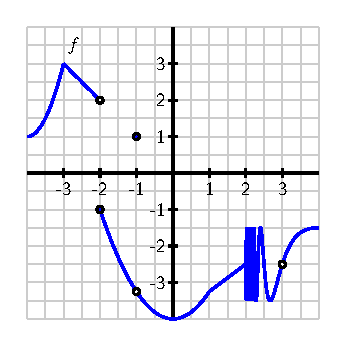
\includegraphics{figures/1_7_PA1.eps}
\caption{The graph of $y = f(x)$.} \label{F:1.7.PA1}
\end{center}
\end{figure}
\ba
	\item For each of the values $a = -3, -2, -1, 0, 1, 2, 3$, determine whether or not $\ds \lim_{x \to a} f(x)$ exists.  If the function has a limit $L$ at a given point, state the value of the limit using the notation $\ds \lim_{x \to a} f(x) = L$.  If the function does not have a limit at a given point, write a sentence to explain why.
	\item For each of the values of $a$ from part (a) where $f$ has a limit, determine the value of $f(a)$ at each such point.  In addition, for each such $a$ value, does $f(a)$ have the same value as $\ds \lim_{x \to a} f(x)$?
	\item For each of the values $a = -3, -2, -1, 0, 1, 2, 3$, determine whether or not $f'(a)$ exists.  In particular, based on the given graph, ask yourself if it is reasonable to say that $f$ has a tangent line at $(a,f(a))$ for each of the given $a$-values.  If so, visually estimate the slope of the tangent line to find the value of $f'(a)$.
\ea
\end{pa} 

\afterpa

